\chapter{Resultados}
\chaptermark{Resultados}

\section{Aplicación de referencia}

Como ya se ha descrito en anteriores secciones, los sistemas guest desarrollados para evaluar el rendimiento de los hipervisores Xen y Jailhouse, tienen como obetivo medir la latencia introducida en la atención a interrupciones debida a la utilizaión de los mismos. \\
Con objeto de poder comparar los resultados obtenidos, es necesario establecer unos datos de partida, es decir, caracterizar el comportamiento del sistema cuando no hay ningún hipervisor. Para ello, se ha desarrollado una aplicación que se ejecuta de forma nativa en la tarjeta electrónica sin ningún sistema operativo ni hipervisor, lo que se conoce tradicionalmente por una aplicación baremetal.\\

El código fuente de esta aplicación es exactamente el mismo que el del DomU de la sección \ref{subsect:xen_app_baremetal} y funcionalmente igual al de la celda baremetal de la sección \ref{jailhouse:app_baremetal}. Su contenido de puede describir de la siguiente forma:
\begin{itemize}
  \item Configuración de los siguientes elementos:
  \begin{itemize}
    \item Temporizador en modo \acrshort{PWM} a fin de generar una señal periódica de 50 ms, que servirá de entrada al siguiente bloque como aparece en la figura \ref{fig:resultados:baremetal_1}.
    \item Bloque \acrshort{GPIO} para generar una interrupción con cada cambio de estado en en la entrada.
    \item Bloque \acrshort{GPIO} que activa la captura indicando que la interrupción ha sido atendida.
    \item Temporizador en modo captura para guardar la referencia de tiempo del instante en el que se produce la interrupción y el instante en el que es atendida.
  \end{itemize}
  \item Rutina de atención a la interrupción en la que se activa una salida del bloque \acrshort{GPIO}.
  \item Bucle principal en el que se accede a los registros del temporizador en modo captura para calcular la diferencia de tiempos.\\
\end{itemize}

\begin{figure*}[h]
  \centering
  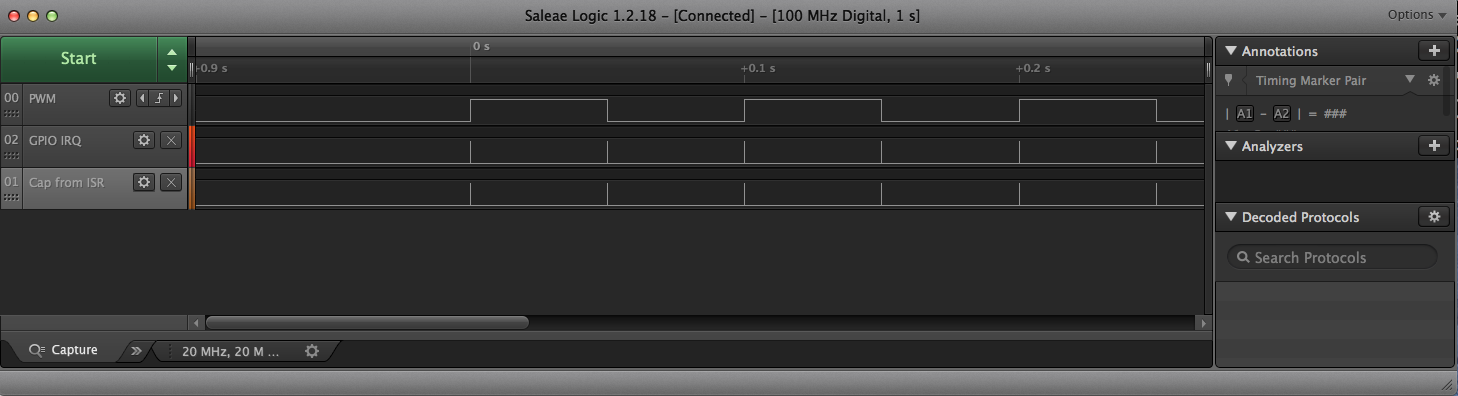
\includegraphics[width=1.0\textwidth]{recursos/baremetal_1.png}
  \caption{Señales de PWM e interrupción}
  \label{fig:resultados:baremetal_1}
\end{figure*}

Las señales que aparecen en las figuras \ref{fig:resultados:baremetal_1}, \ref{fig:resultados:baremetal_2}, \ref{fig:resultados:jailhouse} y \ref{fig:resultados:xen} son las siguientes:
\begin{itemize}
  \item Salida del temporizador en modo \acrshort{PWM}.
  \item Señal de interrupción generada por el bloque \acrshort{GPIO} \textit{axi\_gpio\_0} de la figura \ref{fig:vivado_1}.
  \item Activación de la señal del bloque \acrshort{GPIO} \textit{axi\_gpio\_3} de la figura \ref{fig:vivado_1} producida en la \acrshort{ISR}.
\end{itemize}

Al ejecutar la aplicación de refenrencia, como se puede observar en la figura \ref{fig:resultados:baremetal_2}, la latencia ronda los 360 ns.\\

\begin{figure*}[!h]
  \centering
  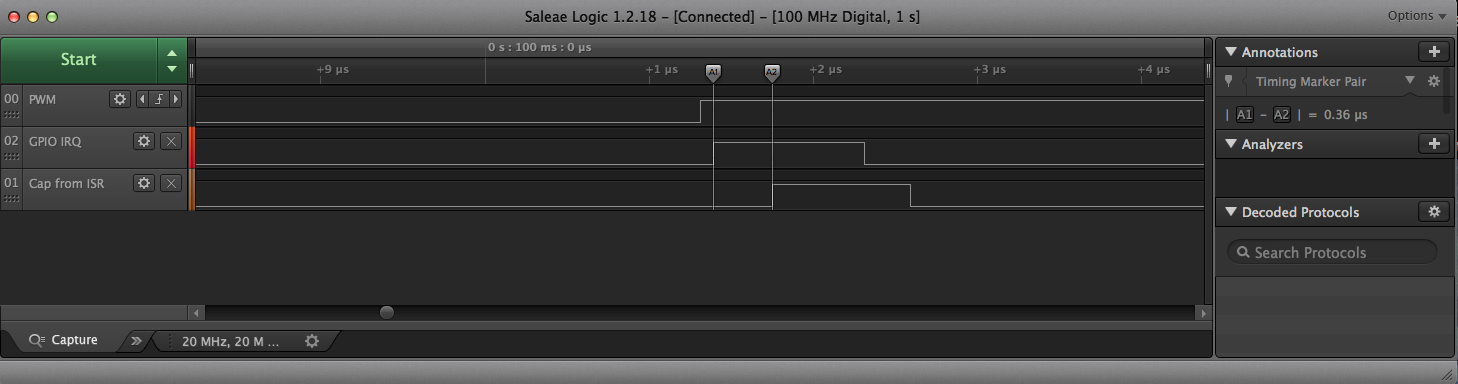
\includegraphics[width=1.0\textwidth]{recursos/baremetal_2.png}
  \caption{Latencia de interrupción en aplicación de referencia}
  \label{fig:resultados:baremetal_2}
\end{figure*}

Los valores obtenidos en una muestra de 256 interrupciones aparecen en la tabla \ref{table:results_baremetal}. \\
\begin{table}[!ht]
  \centering
	\begin{tabular}{ |c|c|c|c| }
		\hline
    Mínimo          & Media      & Máximo  & Desvicación típica  \\
    \hline
    360 ns         & 360.08 ns      & 380 ns    & 1.27 ns	   \\
    \hline
	\end{tabular}
	\caption{Tiempos medidos para aplicación de referencia}
  \label{table:results_baremetal}
\end{table}

\section{Aplicación baremetal en celda Jailhouse}

Los resultados para Jailhouse del test descrito en la sección \ref{test:jailhouse} se muestran en la figura \ref{fig:resultados:jailhouse} y en la tabla \ref{table:results_jailhouse}.\\

\begin{figure*}[!h]
  \centering
  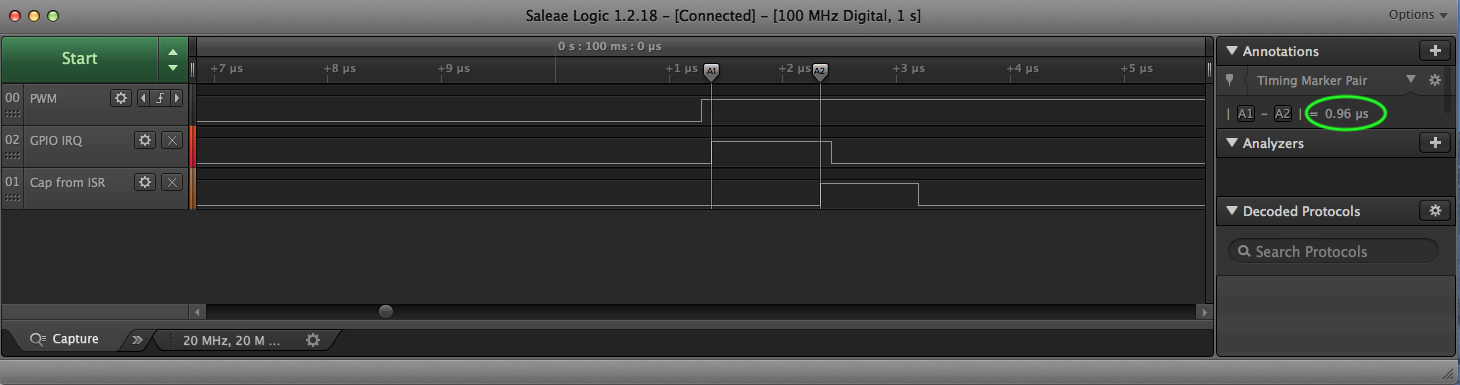
\includegraphics[width=1.0\textwidth]{recursos/jailhouse_1_saleae.png}
  \caption{Latencia de interrupción en Jailhouse}
  \label{fig:resultados:jailhouse}
\end{figure*}

\begin{table}[!ht]
  \centering
	\begin{tabular}{ |c|c|c|c| }
		\hline
    Mínimo          & Media      & Máximo  & Desvicación típica  \\
    \hline
    950 ns         & 958.40 ns      & 1050 ns    & 5.85 ns	   \\
    \hline
	\end{tabular}
	\caption{Tiempos medidos para Jailhouse}
  \label{table:results_jailhouse}
\end{table}

\section{Aplicación baremetal en DomU de Xen}

En el caso de Xen, los resultados obtenidos de la prueba definida en la sección \ref{section:text_xen} aparecen reflejados en la tabla \ref{table:results_xen} y la figura \ref{fig:resultados:xen}.\\

\begin{figure*}[!h]
  \centering
  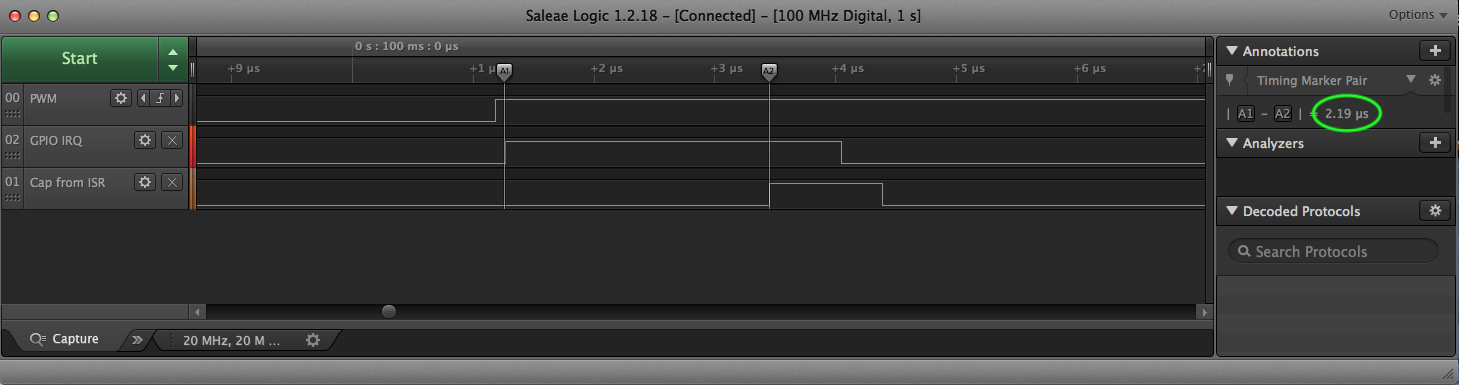
\includegraphics[width=1.0\textwidth]{recursos/xen_1_saleae.png}
  \caption{Latencia de interrupción en Xen}
  \label{fig:resultados:xen}
\end{figure*}

\begin{table}[!ht]
  \centering
	\begin{tabular}{ |c|c|c|c| }
		\hline
    Mínimo          & Media      & Máximo  & Desvicación típica  \\
    \hline
    2130 ns         &  2182.65 ns     & 2320 ns    & 30.32 ns	   \\
    \hline
	\end{tabular}
	\caption{Tiempos medidos para Xen}
  \label{table:results_xen}
\end{table}

\section{Resumen de resultados}
\pgfplotstableread[row sep=\\,col sep=&]{
    interval & carT & carD & carR \\
    Mínimo    & 360  & 950  & 2130  \\
    Media    & 360.08  & 958.40  & 2182.65  \\
    Máximo    & 380  & 1050  & 2320  \\
    }\mydatabig

\pgfplotstableread[row sep=\\,col sep=&]{
    interval & carT & carD & carR \\
    Desviación    & 1.27  & 5.85  & 30.32  \\
    }\mydatadesv


\begin{minipage}[b]{.5\linewidth}
  \begin{adjustbox}{width=\linewidth}
    \begin{tikzpicture}
      \begin{axis}[
        every axis plot post/.style={/pgf/number format/fixed},
        ybar,
        symbolic x coords={Mínimo,Media,Máximo},
        xtick=data,
        axis x line=bottom,
        enlarge x limits=0.2,
        hide y axis,
        nodes near coords,
        ]
        \addplot table[x=interval,y=carT]{\mydatabig};
        \addplot table[x=interval,y=carD]{\mydatabig};
        \addplot table[x=interval,y=carR]{\mydatabig};
        \legend{Baremetal, Jailhouse, Xen}
      \end{axis}
    \end{tikzpicture}
  \end{adjustbox}
\end{minipage}

\begin{minipage}[b]{.5\linewidth}
  \begin{adjustbox}{width=\linewidth}
    \begin{tikzpicture}
      \begin{axis}[
        ybar,
        symbolic x coords={Desviación},
        xtick=data,
        hide y axis,
        axis x line=bottom,
        ytick=\empty,
        nodes near coords,
        ]
        \addplot table[x=interval,y=carT]{\mydatadesv};
        \addplot table[x=interval,y=carD]{\mydatadesv};
        \addplot table[x=interval,y=carR]{\mydatadesv};
        %\legend{Baremetal, Jailhouse, Xen}
      \end{axis}
    \end{tikzpicture}
  \end{adjustbox}
\end{minipage}
